\chapter{Planificación y costes}

%Definir claramente de acuerdo con el tutor los “paquetes de trabajo” (PTs), identificando claramente los entregables resultantes de cada uno de ellos. Esto definirá claramente los resultados del proyecto. Pueden usarse Diagramas de Gantt o cualquier herramienta o metodología siempre que facilite la visualización secuencial y dependencias entre los PT. En este mismo capítulo se incluir un presupuesto –ajustado en lo posible a la realidad- que incluya recursos humanos y materiales, así como cualquier dato que determine la viabilidad del proyecto.

En este capítulo se van a definir las diferentes etapas del proyecto mediante diagramas de Gantt realizados con la aplicación \textit{OpenProj}. Además se incluye el presupuesto necesario para la realización de dicho proyecto.

\section{Planificación}

La figura \ref{fig:gantt-ini} muestra la propuesta inicial de las etapas del proyecto, donde se diferencian varios bloques, el primero sería el de estudio e introducción a lo que se va a realizar en el proyecto, que comprendería desde septiembre hasta finales de noviembre, el segundo bloque o implementación del algoritmo, desde mediados de noviembre hasta finales de diciembre, el tercer bloque contiene todo lo referente a la \textit{blockchain} ARK siendo el grueso del proyecto, comienza a finales de enero hasta mayo. Y por último la parte de las de las pruebas, son 10 días en mayo. La memoria se ha redactado durante todo el proyecto.\\

Pero no todo ha sido como se había planificado, puesto que han surgido algunos imprevistos. A la hora de realizar la implementación del algoritmo \acrshort{uov} en \texttt{python} no existe una biblioteca para trabajar con matrices y cuerpos finitos al mismo tiempo, así ha aumentado el tiempo que se iba a dedicar al algoritmo. Además el trabajo con ARK ha sido más tedioso del esperado, retrasando los tiempos programados.\\

El diagrama de Gantt real se ha dividido en aproximadamente cuatrimestres para que se visualice mejor, la figura \ref{fig:gantt-real-1} muestra las fases de estudio e implementación hasta febrero, la figura \ref{fig:gantt-real-2} incluye el tiempo dedicado a terminar la implementación y realizar el trabajo con ARK hasta julio y la figura \ref{fig:gantt-real-3} contiene el tiempo restante de trabajo con ARK desde julio hasta noviembre, además del periodo de pruebas.


%\vspace*{2cm}
\begin{landscape}
	\begin{figure}[h]
		\centering
		\hspace*{-2cm}
		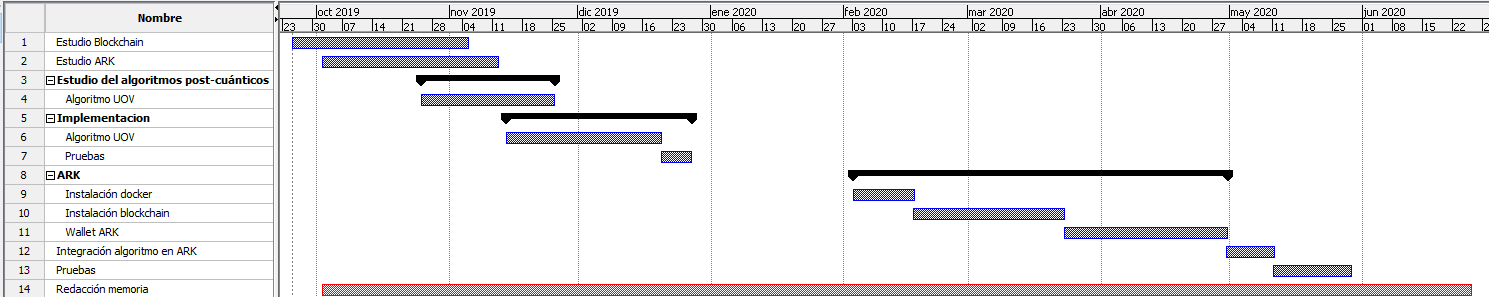
\includegraphics[width=20cm,height=6cm]{figuras/Gantt_ini.png}
		\caption{Diagrama de Gantt inicial}
		\label{fig:gantt-ini}
	\end{figure}
\end{landscape}




\begin{figure}[H]
	\centering
	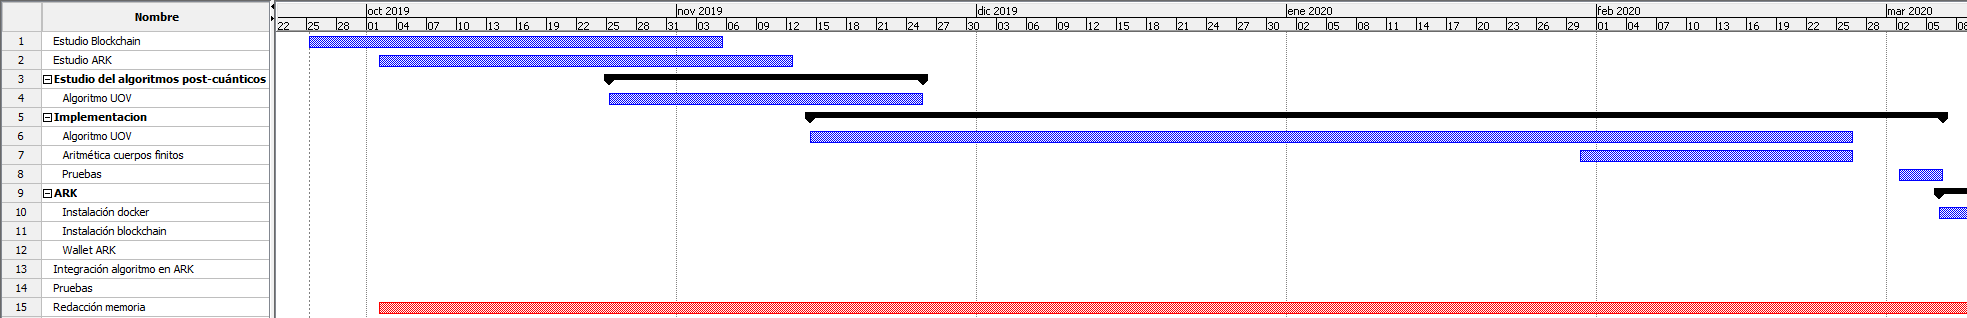
\includegraphics[width=13cm,height=5cm]{figuras/Gantt_1.png}
	\caption{Diagrama de Gantt real. Parte I}
	\label{fig:gantt-real-1}
\end{figure}

\begin{figure}[H]
	\centering
	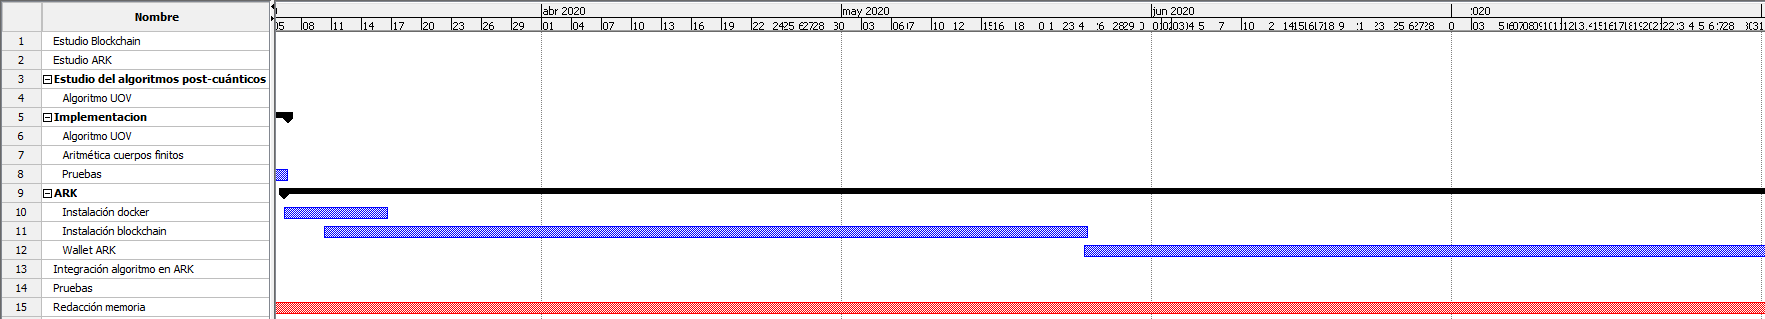
\includegraphics[width=13cm,height=5cm]{figuras/Gantt_2.png}
	\caption{Diagrama de Gantt real. Parte II}
	\label{fig:gantt-real-2}
\end{figure}

\begin{figure}[H]
	\centering
	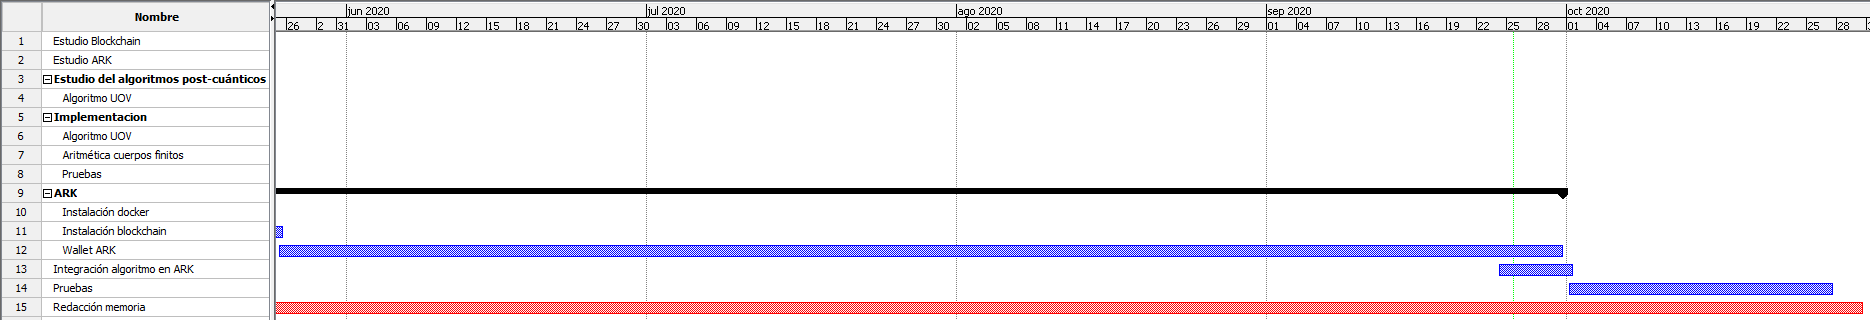
\includegraphics[width=13cm,height=5cm]{figuras/Gantt_3.png}
	\caption{Diagrama de Gantt real. Parte III}
	\label{fig:gantt-real-3}
\end{figure}


\section{Costes}

A continuación se va a detallar el presupuesto invertido en el desarrollo del proyecto. Los costes del mismo se van a desglosar en recursos humanos, costes indirectos, costes directos y viajes.\\


%\vspace*{0.5cm}

Los costes en recursos humanos se van a dividir en dos tablas, una para los tutores, tabla \ref{tab:coste-rh-tut}, y otra para la alumna, tabla \ref{tab:coste-rh-alum}.\\

La tabla \ref{tab:coste-rh-tut} muestra los costes de recursos humanos de los tutores. Para ello se han calculado las horas dedicadas a cada apartado y se ha estimado que el precio de cada hora de trabajo de los tutores es de $20$\euro. Las hora se han divido en tres grandes bloques, estudio, desarrollo y uno general, este último corresponde al tiempo dedicado a la corrección de la memoria y las tutorías con la alumna.\\



\begin{table}[H]
	\begin{center}
	\centering
	\resizebox{\linewidth}{!}{
	\begin{tabular}{p{0.6\linewidth} p {0.15\linewidth}p{0.15\linewidth}}
		\textbf{Descripción del coste} & \textbf{Cantidad (horas)} & \textbf{Coste total (\euro)} \\
		\toprule
		Bloque de estudio\\
		\toprule
		Selección del proyecto & 5 & 100\\[0.5ex]
		Estudio ARK & 6 & 120\\
		Estudio algoritmo UOV & 15 & 300 \\[0.5ex]
		\toprule
		Bloque de desarrollo\\
		\toprule
		Algoritmo UOV & 10 & 200\\[0.5ex]
		Instalación \textit{blockchain} & 3 & 60\\[0.5ex]
		Integración algoritmo & 14 & 280\\[0.5ex]
		\toprule
		Bloque general\\
		\toprule
		Corrección memoria & 12 & 240\\[0.5ex]
		Reuniones & 43 & 860\\[0.5ex]
		\bottomrule
		TOTAL (\euro) & & 2.160\\
	\end{tabular}}
	\end{center}
	\caption{Desglose de los costes en recursos humanos de los tutores}
	\label{tab:coste-rh-tut}
\end{table}
\vspace{0.6cm}

La tabla \ref{tab:coste-rh-alum} muestra los costes de recursos humanos  de la alumna de la misma forma se ha dividido en tres bloques, estudio, desarrollo y uno general, el último corresponde al tiempo dedicado a la memoria y a las reuniones con ambos tutores. Se ha estimado que el precio por cada hora de trabajo de la alumna es de 12\euro.\\

\begin{table}[H]
	\begin{center}
	\centering
	\resizebox{\linewidth}{!}{
	\begin{tabular}{p{0.6\linewidth} p {0.15\linewidth}p{0.15\linewidth}}
		\textbf{Descripción del coste} & \textbf{Cantidad (horas)} & \textbf{Coste total (\euro)} \\
		\toprule
		Bloque de estudio\\
		\toprule
		Estudio tecnología blockchain & 32 & 384\\[0.5ex]
		Estudio ARK & 50 & 600\\
		Estudio algoritmos post-cuánticos & 28 & 336\\[0.5ex]
		\toprule
		Bloque de desarrollo\\
		\toprule
		Algoritmo UOV & 24 & 288\\[0.5ex]
		Aritmetica cuerpos finitos & 23 & 276\\[0.5ex]
		Instalación docker & 20 & 240\\[0.5ex]
		Instalación \textit{blockchain} & 20 & 240\\[0.5ex]
		Wallet ARK & 25 & 300\\[0.5ex]
		Integración algoritmo & 60 & 720\\[0.5ex]
		Pruebas & 16 & 192\\[0.5ex]
		\toprule
		Bloque general\\
		\toprule
		Redacción memoria & 70 & 840\\[0.5ex]
		Corrección memoria & 19 & 228\\[0.5ex]
		Reuniones & 43 & 516\\[0.5ex]
		\bottomrule
		TOTAL (\euro) & & 5.160\\
	\end{tabular}}
	\end{center}
	\caption{Desglose de los costes en recursos humanos de la alumna}
	\label{tab:coste-rh-alum}
\end{table}
\vspace{0.6cm}

Los costes indirectos corresponden a la electricidad y alquiler de la oficina como estos gastos no se pueden estimar correctamente se va a destinar un $10\%$ del total del proyecto. En este caso corresponde a $755,24$\euro \label{par:coste-ind}.\\


En los costes directos se van a meter los gatos en material de oficina, material informático y servicio de mantenimiento, veáse la tabla \ref{tab:coste-di}. Este último incluye el precio de un nuevo disco de memoria interno, ya que ha sido necesario aumentar la memoria del portátil durante el desarrollo del proyecto.

El material informático utilizado ha sido únicamente el equipo de trabajo, un portatil ASUS TP$300$L. Teniendo en cuenta que el precio de adquisición del ordenador fue de $750,00$\euro\ y suponiendo que la vida media de un ordenador es de unos 6 años, entonces el gasto que corresponde durante los 13 meses del desarrollo del proyecto es de  $135,41$\euro.\\


\begin{table}[H]
	\begin{center}
	\centering
	\begin{tabular}{p{0.4\linewidth} p {0.2\linewidth}}
		\textbf{Descripción del coste} & \textbf{Cantidad} \\
		\toprule
		Material de oficina & 30\euro\\[0.5ex]
		Material informático & 135,41\euro\\[0.5ex]
		Servicio de mantenimiento & 45\euro\\[0.5ex]
		\bottomrule
		TOTAL (\euro) & 210,4 \euro\\
	\end{tabular}
	\end{center}
	\caption{Desglose de los costes directos}
	\label{tab:coste-di}
\end{table}


En los costes en viajes solo ha sido necesario incluir los viajes a la escuela de informática para las reuniones con el tutor, puesto que a la facultad de ciencias no era necesario coger un transporte. Solo se han realizado viajes en el primer cuatrimestre del curso $2019$-$2020$, ya que el resto de las reuniones han sido de forma virtual, obteniendo un total de costes de $22$\euro \label{par:coste-via}.\\


\begin{table}[H]
	\begin{center}
	\centering
	\begin{tabular}{p{0.4\linewidth} p {0.2\linewidth}}
		\textbf{Tipo de costes} & \textbf{Cantidad} \\
		\toprule
		Recursos humanos & 7.320\euro\\[0.5ex]
		Indirectos & 755,24\euro\\[0.5ex]
		Directos & 210,40\euro\\[0.5ex]
		Viajes & 22\euro\\[0.5ex]
		\bottomrule
		TOTAL (\euro) & 8.307,64\euro\\
	\end{tabular}
	\end{center}
	\caption{Presupuesto gastos previstos desglosado}
	\label{tab:coste-total}
\end{table}

Una vez que hemos calculado todos los gastos posibles, tabla \ref{tab:coste-total}, vamos a añadir un margen de contingencia del $5\%$ para posibles imprevistos del proyecto. Hemos obtenido que los gastos previstos serán de 8.307,64\euro, por tanto el margen de contigencia será de 415,38\euro, así el presupuesto final sera de 8.723,02\euro\label{par:coste-impr}.


\begin{table}[H]
	\begin{center}
	\centering
	\begin{tabular}{p{0.6\linewidth} p {0.2\linewidth}}
		\textbf{Tipo de costes} & \textbf{Cantidad} \\
		\toprule
		Recursos humanos, tabla \ref{tab:coste-rh-tut} y tabla \ref{tab:coste-rh-alum} & 7.320\euro\\[0.5ex]
		Indirectos, párrafo \ref{par:coste-ind} & 755,24\euro\\[0.5ex]
		Directos, tabla \ref{tab:coste-di} & 210,40\euro\\[0.5ex]
		Viajes, párrafo \ref{par:coste-via} & 22\euro\\[0.5ex]
		Gastos imprevistos, párrafo \ref{par:coste-impr} & 415,38\euro\\[0.5ex]
		\bottomrule
		TOTAL (\euro) & 8.723,02\euro\\
	\end{tabular}
	\end{center}
	\caption{Presupuesto total desglosado}
	\label{tab:coste-total}
\end{table}